\documentclass{article}[hidelinks]
\usepackage{changepage}% http://ctan.org/pkg/changepage
\usepackage{lipsum}% http://ctan.org/pkg/lipsum
\usepackage[utf8]{inputenc}
\usepackage[a4paper]{geometry}
\usepackage{amsmath}
\usepackage{rotating}
\usepackage{setspace}
\usepackage{graphicx}
\usepackage{dcolumn}
\usepackage{booktabs}
\usepackage[hidelinks]{hyperref}
\usepackage{natbib}
\usepackage{threeparttable} %Adding notes to tables
\usepackage[export]{adjustbox} % for figures
\usepackage[usenames,dvipsnames]{color}


%Packages for Caption
%https://tex.stackexchange.com/questions/134399/how-to-center-table-caption-that-includes-a-newline
\usepackage{caption}
\newcommand{\source}[1]{\vspace{-3pt} \caption*{ Source: {#1}} }
\usepackage{varwidth}
\DeclareCaptionFormat{myformat}{%
  % #1: label (e.g. "Table 1")
  % #2: separator (e.g. ": ")
  % #3: caption text
  \begin{varwidth}{\linewidth}%
    \centering
    #1#2#3%
  \end{varwidth}%
}

% Bibliography commands
\bibliographystyle{apsr}

\usepackage[hyphenbreaks]{breakurl}
\usepackage[hyphens]{url}

\setcounter{biburllcpenalty}{7000}
\setcounter{biburlucpenalty}{8000}

\usepackage{hyperref}
\hypersetup{
breaklinks=true,
colorlinks=false,
citebordercolor={.2 .2 .6},
urlbordercolor={.0 1.0 1.0}
}

% Kopf- und Fußzeile
\usepackage{fancyhdr}
\pagestyle{fancy}
\pagestyle{fancy}
\fancyhf{}
\rhead{Mapping Moral Beliefs of the World}
\lhead{}
\rfoot{Page \thepage}


\title{\bf Mapping Moral Beliefs of the World - \\
\bigskip
\bigskip
A Descriptive Approach using PCA and Cluster Analysis
}
\author{Lukas Birkenmaier - \url{lukas.birkenmaier@warwick.ac.uk}}
\date{Mon 26th April 2021}
\onehalfspacing
\graphicspath{{images/}}
\pagenumbering{arabic}
\begin{document}
\maketitle
\section*{Abstract}
%TC:ignore
\begin{adjustwidth}{1cm}{1cm}
Individual norms and moral beliefs have long been acknowledged to build the fundament of any modern social structure. Likewise, recent survey data shows that, despite ongoing globalization tendencies, peoples attitudes still vary widely across countries on issues like homosexuality, divorce or bribery. In this paper, I aim to explore this issue by mapping people's moral beliefs across 72 countries and identifying commonalities and differences across moral dimensions. Results from my principal component and cluster analysis show that the two most dominant moral dimensions, namely religious and social order attachments, already explain a lot of variation in people's norms and values across countries. However, more manifold and complex issues, like for instance attitudes on the death penalty, do not necessarily fit into these pattern and may be explained by more specific factors. Ultimately, a total of four distinct groups of countries are identified, which may serve as starting point for further research.
\end{adjustwidth}

\section*{Keywords}
\hspace{1cm} World Values Survey, European Values Survey, PCA, Clustering, Moral Beliefs
%TC:endignore
\newpage \tableofcontents 
\newpage \listoffigures

%%%%%%%%%%%%%%%% Begin of Document %%%%%%%%%%%%%%%%%%%%%%%%
\section{Introduction}

In the last few decades, globalization tendencies have brought tremendous changes and social upheavals for humans across the globe. Especially the rise of modern information and communication technologies can be directly linked to increased exchanges of cultural concepts, normative standards and moral beliefs \citep{Adamczyk.2013}. However, results from recent cross-country surveys show that people are still closely connected to the ethical standards and norms of their own cultural background. In this paper, I will take a rather descriptive approach to get a better understanding of this phenomenon. 
Using data from both the World Values Survey \citep{Haerpfer.2020} and the European Values Survey \citep{luijkx2021european}, I aim to explore differences in peoples norms and beliefs across countries. Hence, I want to answer the question on how certain moral beliefs relate to each other, and how countries might be grouped into similar clusters with shared moral beliefs

Doing so, the next section will shortly summarize the current state of knowledge on why people´s personal attitudes on norms and ethics vary, and which factors might be influential in shaping these opinions in the first place. Section three will then introduce my research design, followed by the presentation of my main results in section four and a concise conclusion in section five.

\section{Theory}
\subsection{Ethics and Norms on the Individual and Group Level}

Personal attitudes, such as individual norms, beliefs and values, provide the most basic building blocks of a person’s “individual culture” \cite[~p.194]{Chai.2009}. These personal attitudes, which I will use synonymously throughout this paper, then provide the fundament of any societal order \citep{Jelen.2003}. However, the causal relationships between norms and social structures remain complex and structurally unclear. This is due to the fact that people generate social structures and rules based on their personal beliefs. At the same time, however, these structures and norms do socialize individuals and shape their personal moral compass \citep{Chai.2009}. 
Eventually, researcher will likely never succeed in fully understanding the causal mechanisms behind these interactions. Nevertheless, on the group level, it can be observed that individual ethics and norms have an enormous impact on societal rules and norms, which emphasized the relevance for researchers to understand their origin and dissemination across different cultures and countries. 

\bigskip
\subsection{On the Origin of Ethics and Norms}

Where do ethical values and norms come from? Evaluating the factors that underlay common moral principles, the relevant literature points to two major explanations on what shapes moral beliefs and ethics. First, one strand of literature explains the emergence of ethics and moral principles as a direct consequence of a social contract between humans from an early stage on. Based on the ideas of \cite{Hobbes.1968} and \cite{Rousseau.1974}, it is argued that humans, in order to peacefully live side by side in a post state-of-nature society, have to agree on a social order with binding rules and social mechanisms \citep{Midgley.1991}. The consequences of this social contract were then most prominently interpreted by John \cite{Rawls.1971}. In his popular book “A Theory of Justice”, he introduces the veil of ignorance, a concept which describes a temporal state of unawareness about someone social and economic status in life. This state of unknowingness then leads people to agree on rules and social structures, which are inherently fair and ethical. This is caused by the fact that everyone will settle on common rules which ensure as much liberty as possible while having equal opportunity to prosper in life, regardless of someone’s initial societal status. Ultimately, these rules and norms are then adopted by individuals and manifest themselves in social norms and values, such as, for instance, the condemnation of theft and fraud as well as physical violence against other humans.

Second, another strand of literature explains the emergence of ethics and norms based on varying degrees of religiousness and compliance with cultural traditions. According to \cite{Parboteeah.2008}, the link between religion and ethics is directly established trough religious values and provisions. Since religious activities are often linked to formal and informal norms with a freedom/constraint duality, following these norms will provide guidance “to bring [humans] imperfect nature in line with the will of God” \citep[~p.4]{Midgley.1991}. 
\newline Empirically, this link has been examined by several researchers in different contexts. \cite{Jelen.2003}, for instance, find that individual levels of religion are one of the most important predictors for attitudes towards a whole range of issues, such as abortion, gender equality and divorce. Likewise, \cite{Adamczyk.2013} argues that personal religious involvement is a consistent predictor for individual attitudes against salient issues like feminism or abortion. 

\section{Research Design}
\subsection{Data}
To explore differences in norms and ethics across countries and cultures, I rely on data from the joint EVS/WVS 2017-2021 dataset \citep{Joint}. Both the World Values Survey (WVS) \citep{Haerpfer.2020} and the European Values Survey (EVS) \citep{luijkx2021european} are two large-scale, cross-national and longitudinal surveys which systematically explore people's values and beliefs.
Thus, the joint dataset consists of a total of 79 countries and a total number of 127.358 cases, which were collected via face-to-face interviews at the respondents homes between 2017-2021 (for a complete list of countries, cf. Figure \ref{fig:names} in the Appendix) \citep{Gesis}. 
For my analysis, I draw on 13 questions from the ''Values and Norms'' section, which contains answers on whether the respondents belief that actions like stealing property, abortion or homosexuality are justified (cf. Table \ref{tab:variables} in the Appendix). All questions are measured on a 10-item Likert scale, ranging from one (\emph{can never be justified}) to ten (\emph{can always be justified}).
In order to aggregate respondents answers on the country level, I first apply listwise deletion of missing cases \citep{roth1994missing} and then inspect the individual counts for each country to avoid extreme imbalances within the data. Hence, most countries are characterized by a sufficient sample size of over 1000 cases, with Cyprus (n=404) and the Ukraine (n=649) having the least cases. However, after considering all relevant factors like statistical power and expected effect sizes \citep{kadam2010sample}, I decide to keep all countries in my sample and calculate the average values for each category, which results in a final dataset of 72 observations, each representing one single country.

\subsection{Methodology}
In order to examine relationships between norms and moral beliefs across my sample, I first apply principal component analysis (PCA), which is a common statistical technique when assessing high-dimensional datasets. In short, PCA aims to reduce data dimensionality by applying orthogonal linear transformations to extract a set of new orthogonal variables called principal components, where the first few components preserve the majority of data variation \citep{bro2014principal} (cf. Figure \ref{fig:PCA} in the Appendix).
In a second step, I will then group and cluster my samples into distinct groups based on their principal component scores. Therefore, I will apply the popular \emph{K-means} algorithm \citep{likas2003global}, which aims to minimise the within-cluster sum of squares between a set of d-dimensional observations ($x_1$, $x_2$, ..., $x_n$) and a set of clusters (S = {$S_1$, $S_2$, ..., $S_k$}) where $u_i$ is the mean of points in $S_i$ (cf. Equation 1)

\begin{equation}\label{my_first_eqn}
	J=\sum _{{i=1}}^{{k}}\sum _{{{\mathbf  x}_{j}\in S_{{i}}}}{\|{\mathbf  x}_{j}-{\boldsymbol  \mu }_{i}\|^{2}}
\end{equation}


In order to conduct my analysis, I rely on the R-environment \citep{R} and additional packages, most importantly \emph{Tidyverse} \citep{tidy}, \emph{Factoextra} \citep{factoextra} and \emph{NBclust} \citep{NBclust}. A full copy of the code used for this analysis is attached at the end of this document or can directly be downloaded, together with the data, from the authors Github profile \citep{Github}.

\section{Results}
\subsection{Descriptive Statistics and PCA}
Assessing the univariate distribution of norms across countries (cf. Figure \ref{fig:histogramm} in the Appendix), one can observe major differences in approval ratings for different behaviors. Whereas, for instance, \emph{Bribery} ($\not\!\circ \; 1.79$) and \emph{Political violence} ($\not\!\circ \; 1.84$) are often condemned, support for other, more secular, actions like \emph{Homosexuality} ($\not\!\circ \;  4.39$), \emph{Divorce} ($\not\!\circ \; 5.47$) or \emph{Euthanasia} ($\not\!\circ \; 4.38$) varies widely between countries. The correlation table (cf. Figure \ref{fig:correlation} in the Appendix) furthermore provides evidence that support for certain behaviors are correlated. On the one hand, opinions on \emph{Abortion}, \emph{Divorce}, \emph{Homosexuality}, \emph{Suicide}, \emph{Prostitution} and \emph{Casual sex} are often related, just like public opinions on \emph{Fare evasion}, \emph{Tax fraud}, \emph{Bribery} and \emph{Cheating government benefits} on the other hand. This might indicate that both moral dimensions found in the literature reflect themselves within the dataset, namely a religious and a social-contract dimension.
These findings are further strengthened when assessing the results from the PCA analysis. The scree plot \citep{ferre1995selection}) suggests that two components already explain a majority of variance within the data, with the third component mostly explaining variance in support for the \emph{Death penalty} (cf. Figure \ref{fig:pca_eigenvalues} in the Appendix). Figure \ref{fig:biplot} visualises these results, showing that most variables, except for \emph{Death penalty}, have high (negative) contributions to either the secular or antisocial behavior component. Thereby, variation is larger on the religious component, which provides evidence that people opinions within the countries in my dataset differ most on assessment of secular behavior.  
\begin{figure}[h]
    \centering
    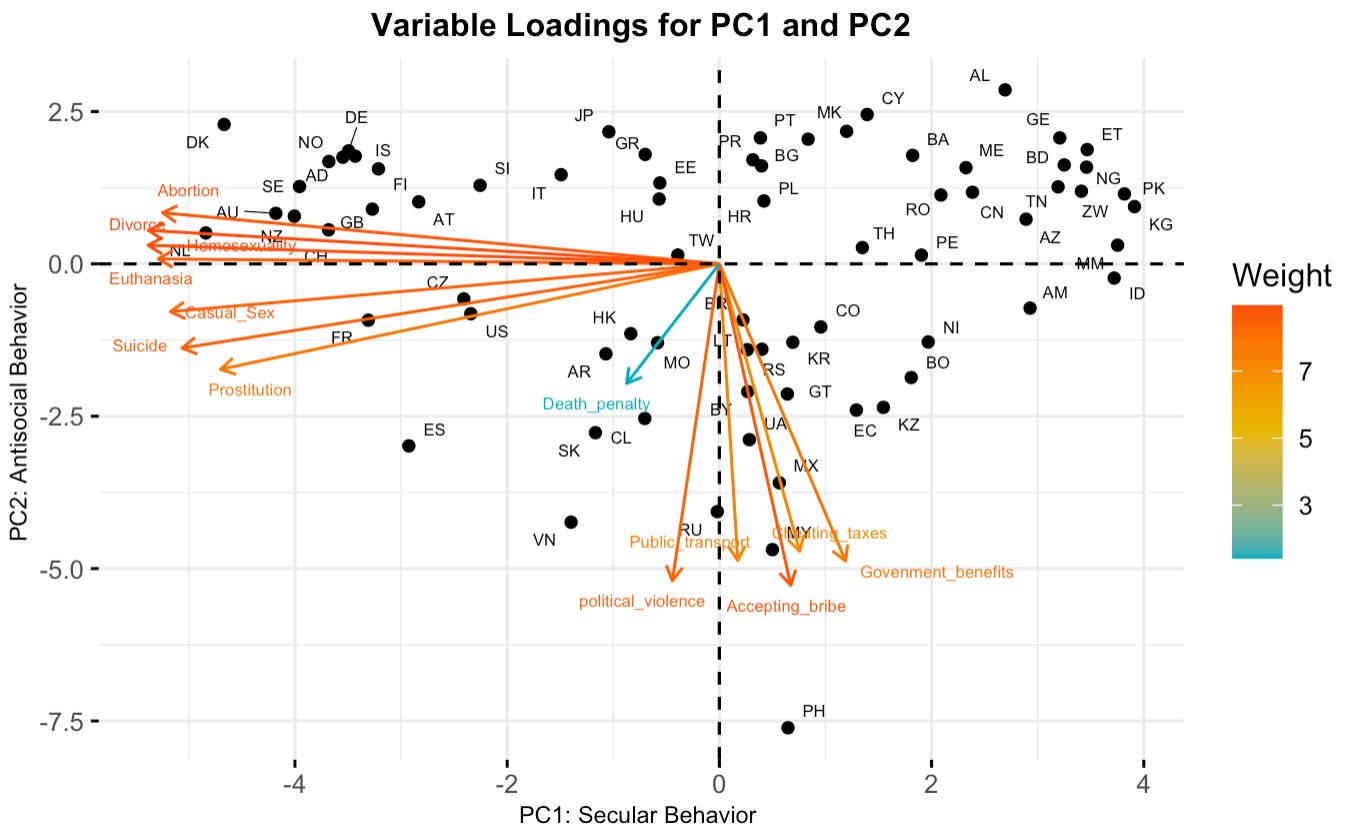
\includegraphics[width=120mm]{variables_PCA_final.png}
    \caption{PCA Biplot on PC1 and PC2}
    \label{fig:biplot}
\end{figure} These findings confirm the main result from my literature review, which primarily identifies a religious and a social dimension of peoples norms and social values. However, there are mixed attitudes towards the \emph{Death penalty}. This seems to be in line with related research on this issue, which provides evidence that people often evaluate the basic human \emph{right to life} detached from their religious or normative moral basis \citep{hood2015death, anckar2004determinants}. To summarize, Figure \ref{fig:final} in the Appendix again displays the correlations of each variable with the most important components.

\subsection{Clustering Algorithm}

In a second step, I furthermore apply the K-means cluster algorithm on the country coordinates for the first three principal components to group my observations into meaningful structures. In order to find the optimal number of clusters, I visually evaluate the scree plot for the within-group sum of squares and use the elbow-method to find the number of clusters where the eigenvalues seem to level off, which results in a total of four clusters. These results are also confirmed when controlling my findings with the \emph{NbClust} function, which compares a total of 30 indices for determining the right number of clusters. 

Table 1 displays the main findings of the algorithm, showing both the total counts and mean for each of the four clusters identified.
 \begin{table}[htb]
  \centering
    \begin{threeparttable}
      \caption{Results Cluster Analysis}
       \centering  %% use this instead of \begin{center}
        \begin{tabular}{l c c c c }
          \toprule
          {Cluster} & {Count}& {\shortstack{PC1:\\ Secular Behavior}} & {\shortstack{PC2:\\ Antisocial Behavior}} & {\shortstack{PC3:\\ Death Penalty}} \\\toprule[1pt]
          Cluster 1 & 13&-0.31 & 0.27 & \textbf{-1.45} \\ 
          Cluster 2 & 21&0.04 & \textbf{-1.27} & 0.03 \\ 
          Cluster 3 & 23& \textbf{1.02} & 0.58 & 0.40 \\ 
          Cluster 4 & 15&\textbf{-1.36} & 0.66 & 0.60 \\ 
          \bottomrule
        \end{tabular}
        \begin{tablenotes}
          %\footnotesize   %% If you want them smaller like foot notes
          \item[a] Note: High values having an absolute value $1\leq$ are highlighted in \textbf{bold}; Since the original variables are negatively correlated with the principal components (cf. Figure \ref{fig:biplot}), negative values can be interpreted as support for the moral dimension and vice versa. 
        \end{tablenotes}
    \end{threeparttable}
  \end{table} The clusters are reasonably balanced and may be be interpreted cautiously in their meaning. Starting with the countries in cluster 1 (e.g. \emph{United States}, \emph{China} and \emph{Japan}), these countries are primarily characterized by high support scores for the death penalty, with only moderate values for PC1 and PC2. Likewise, countries in cluster 2 (e.g. \emph{Colombia}, \emph{Serbia} and \emph{Myanmar}) show high values for antisocial behaviors, whereas they are positioned centrally on the other components. Lastly, countries in cluster 3 (e.g. \emph{Pakistan}, \emph{Romania} and \emph{Indonesia}) and cluster 4 (e.g. \emph{Germany}, \emph{Denmark} and the \emph{Netherlands}) differ primarily in their religious dimension, while moderately disapproving antisocial behavior on PC2 \citep{miller2008religious}. Table \ref{tab:clusters_Assigned} in the Appendix displays a full list of clusters assigned for each country.

\section{Conclusion}

The goal of this paper has been to explore people moral attitudes and emphasize similarities and differences in peoples moral beliefs across countries. Results from my PCA and cluster analysis show that, as expected, religious and social values can be identified as dominant moral dimensions across countries. Furthermore, the assessment of the \emph{Death Penalty} appears to be detached from these dimension, which might be rooted in other factors, such as gender or religious fundamentalism \citep{miller2008religious}. 

Coming to an end, I argue that this paper provides a broad and profound overview and categorisation on dominant values between countries. However, these findings can only serve as a starting point for further research, which should build on these findings and further explore countries characteristics. For instance, researchers could use the principal component loading's as regressors in linear regression models to further explain their impact on important societal characteristics, such as regulatory legal acts or the amount of crimes within a given country.

\newpage \bibliography{citations}
\newpage \section{Appendix}
\captionsetup{format=myformat} %Loading Caption Format
\begin{figure}[h]
    \centering
    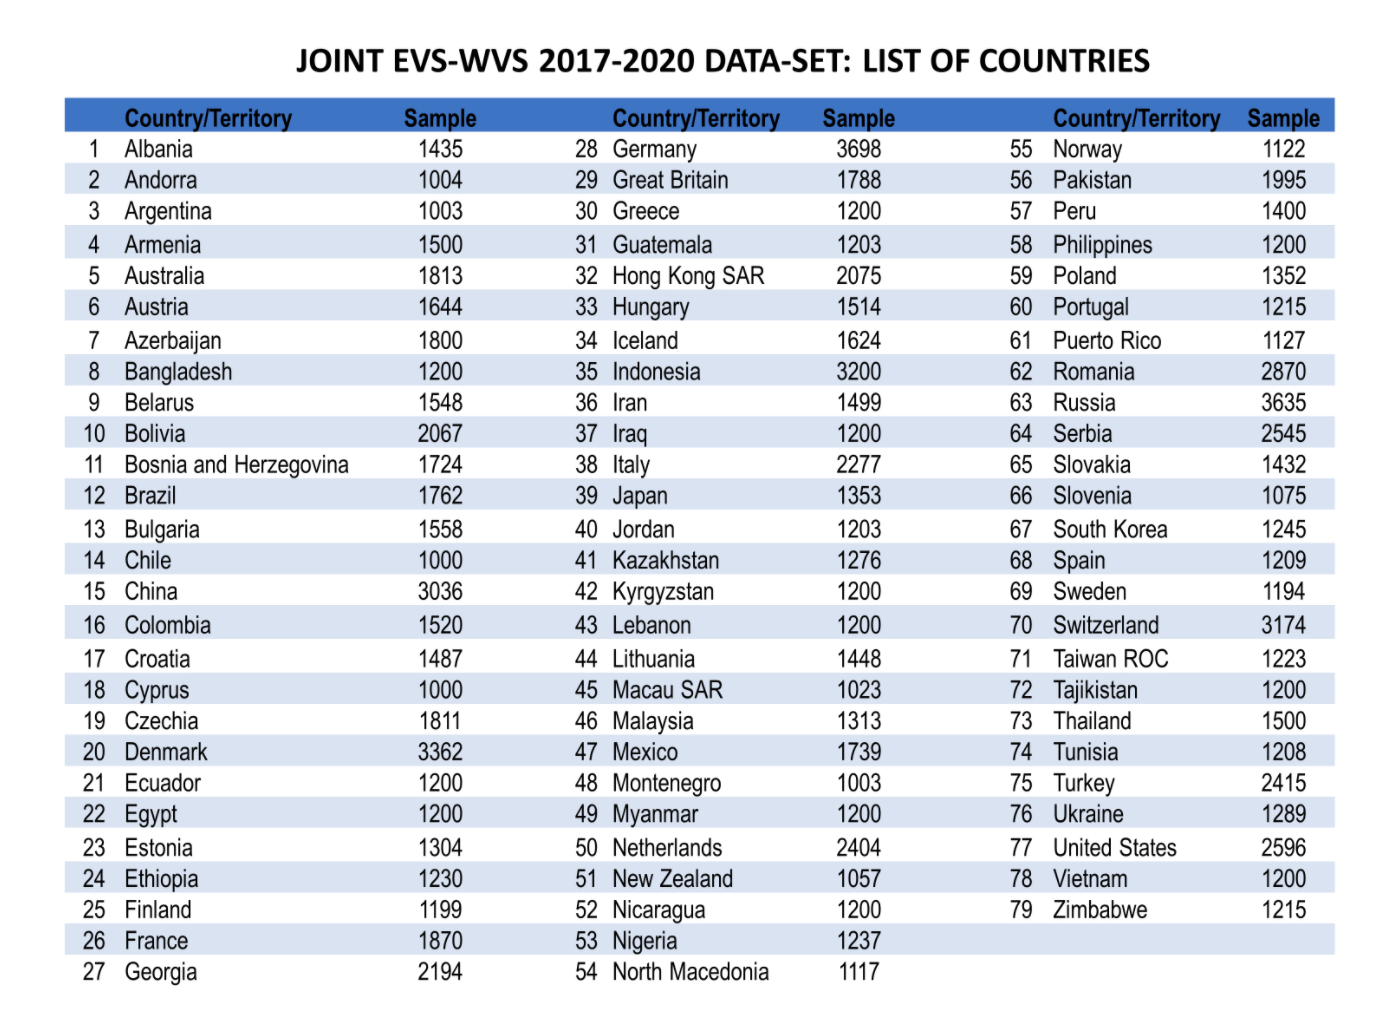
\includegraphics[width=130mm]{Variable List.png}
    \caption{Complete List of Countries}
    \label{fig:names}
    \vspace{-9pt}
    \caption*{Source: https://www.worldvaluessurvey.org/ WVSEVSjoint2017.jsp}
\end{figure}

\begin{table}[htb]
  \centering
    \begin{threeparttable}
      \caption{Potential Ideas for further research}
       \centering  %% use this instead of \begin{center}
        \begin{tabular}{c c l  }
          \toprule
          {No} & {Variable Code}& {Behavior} \\\toprule[1pt]
            1 & F114A & Claiming state benefits which you are not entitled to \\ 
              2 & F116 & Cheating on tax if you have the chance \\ 
              3 & F117 & Someone accepting a bribe in the course of their duties \\ 
              4 & F118 & Homosexuality \\ 
              5 & F120 & Abortion \\ 
              6 & F121 & Divorce \\ 
              7 & F122 & Euthanasia \\ 
              8 & F123 & Suicide \\ 
              9 & F132 & Having casual sex \\ 
              10 & F115 & Avoiding a fare on public transport\\ 
              11 & F119 & Prostitution \\ 
              12 & E290 & Political violence \\ 
              13 & F14402 & Death penalty \\ 
          \bottomrule
        \end{tabular}
            \label{tab:variables}

        \begin{tablenotes}
          %\footnotesize   %% If you want them smaller like foot notes
          \item[a] Question: ''Please tell me for each of the following whether you think it can always be justified, never be justified, or something in between'' 
        \end{tablenotes}
    \end{threeparttable}
  \end{table}


\begin{figure}[h]
    \centering
    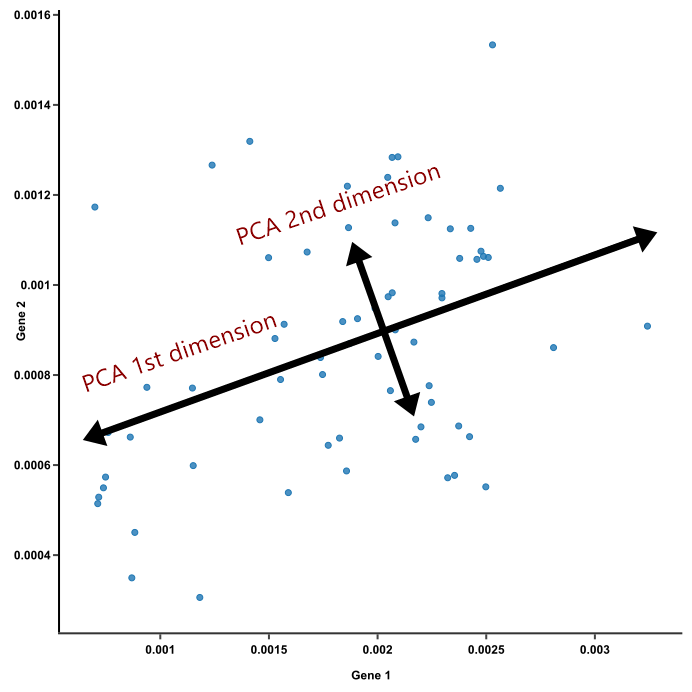
\includegraphics[width=80mm]{PCA.png}
    \caption{Visual Interpretation of Principal Components}
    \label{fig:PCA}
    \vspace{-9pt}
    \caption*{Source: https://blog.bioturing.com/2018/06/14/principal-component- \\ analysis-explained-simply/}
\end{figure}

\begin{figure}[h]
    \centering
    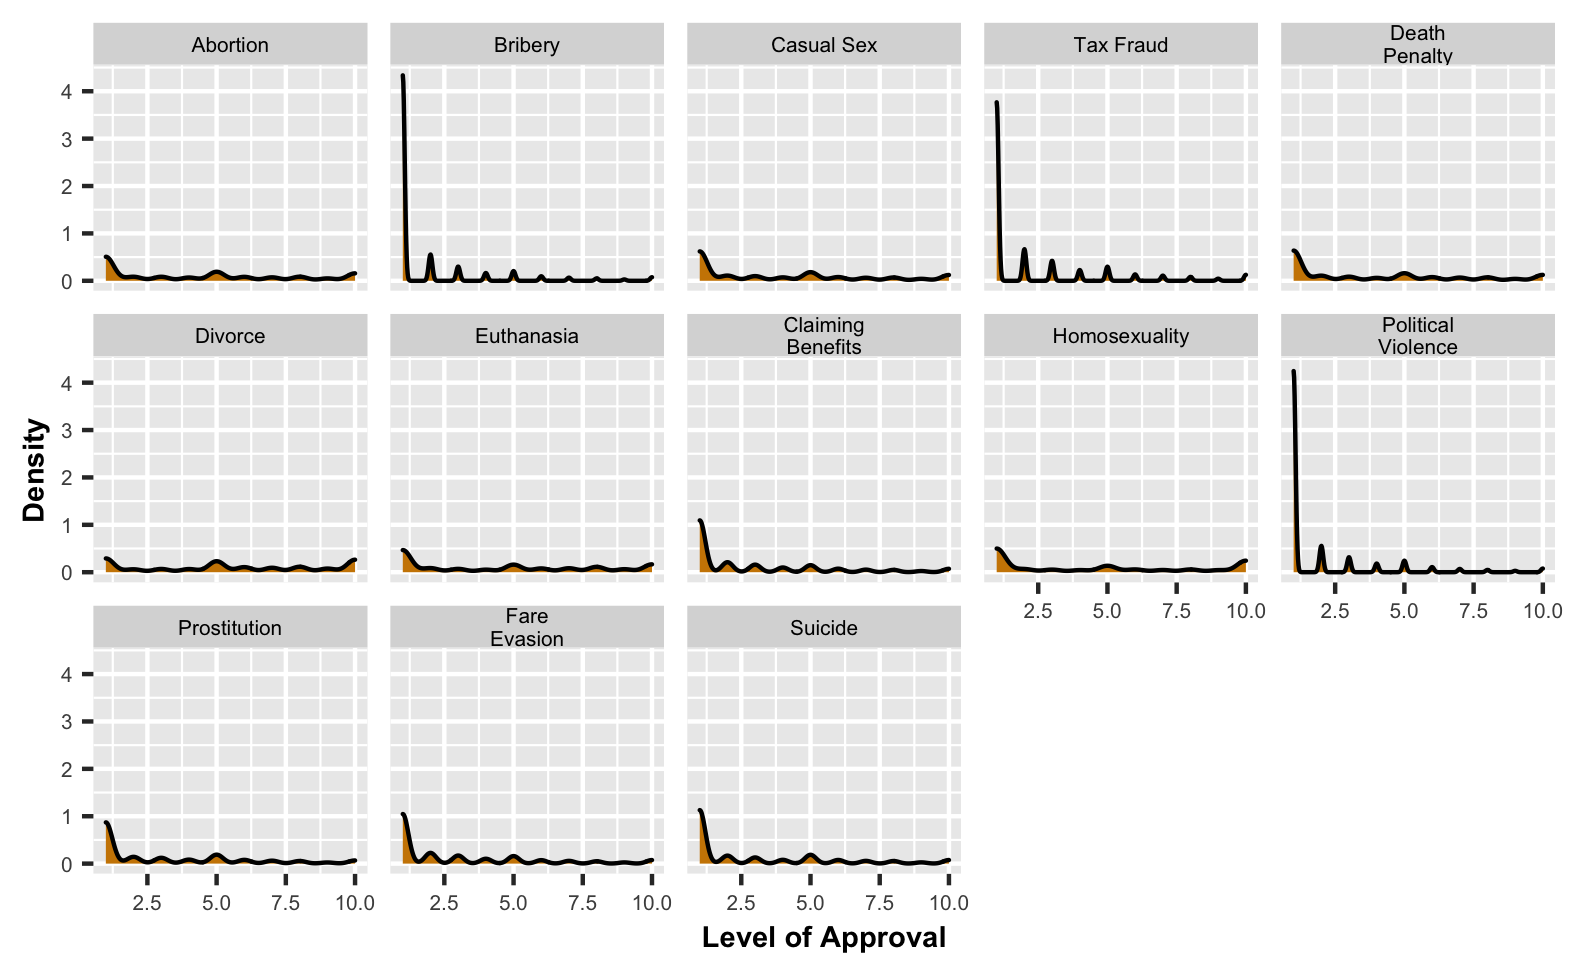
\includegraphics[width=130mm]{histogramm.png}
    \caption{Distribution of Values across Countries (N = 72)}
    \label{fig:histogramm}
    
\end{figure}



\begin{figure}[h]
    \centering
    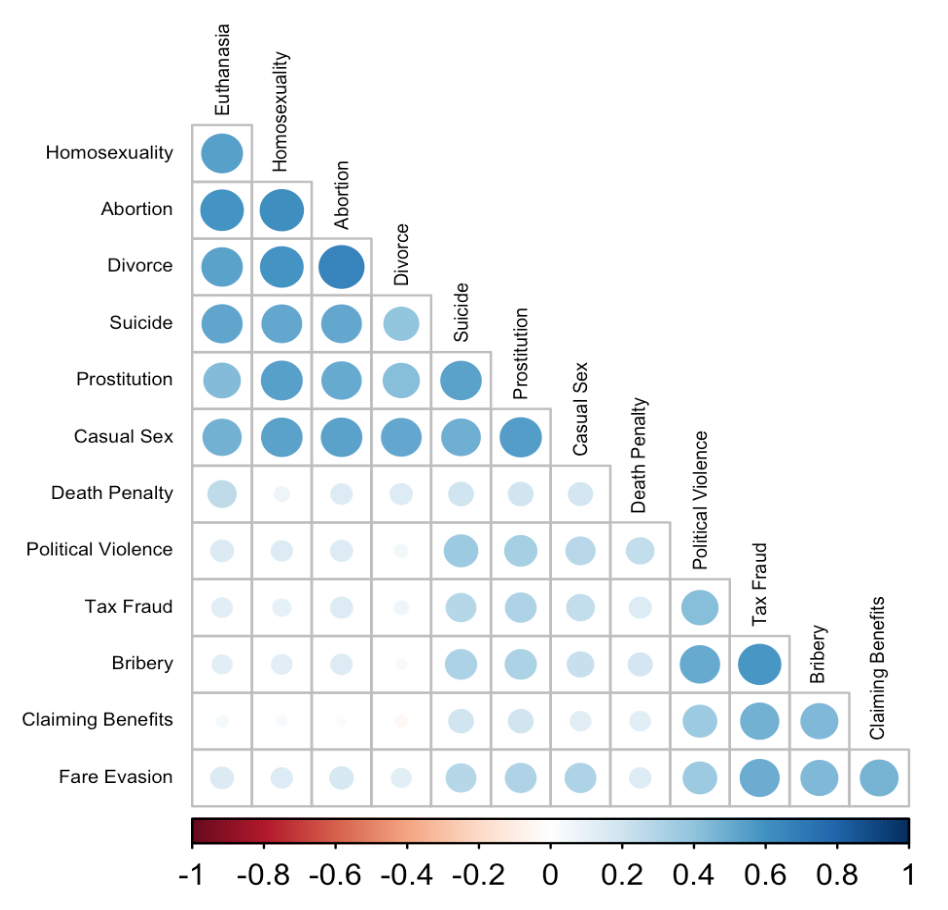
\includegraphics[width=100mm]{correlations.png}
    \caption{Correlations Table (ordered)}
    \label{fig:correlation}
\end{figure}

\begin{figure}[h]
    \centering
    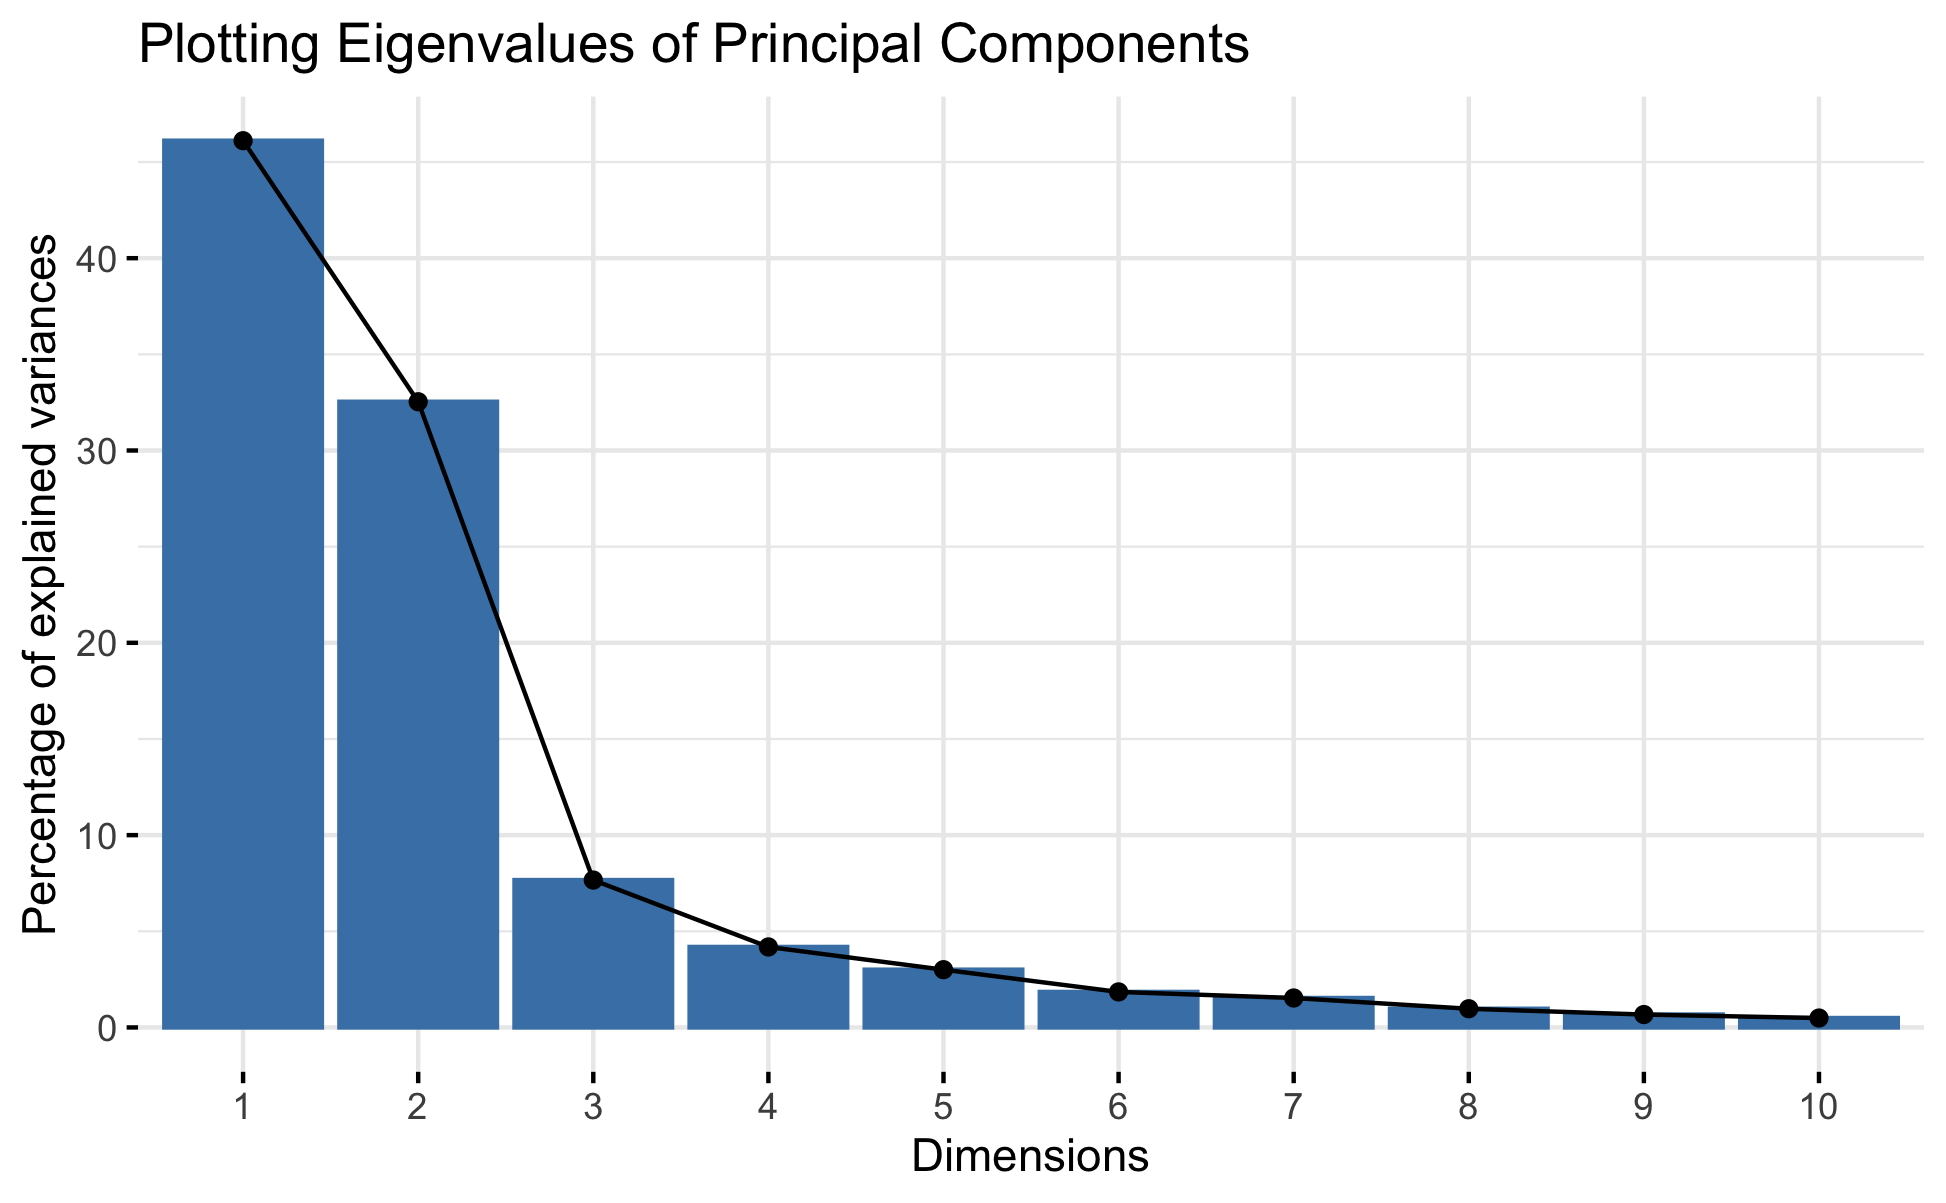
\includegraphics[width=150mm]{components_world.png}
    \caption{Assessing Eigenvalues for PCA}
    \label{fig:pca_eigenvalues}
\end{figure}

\begin{figure}[h]
    \centering
    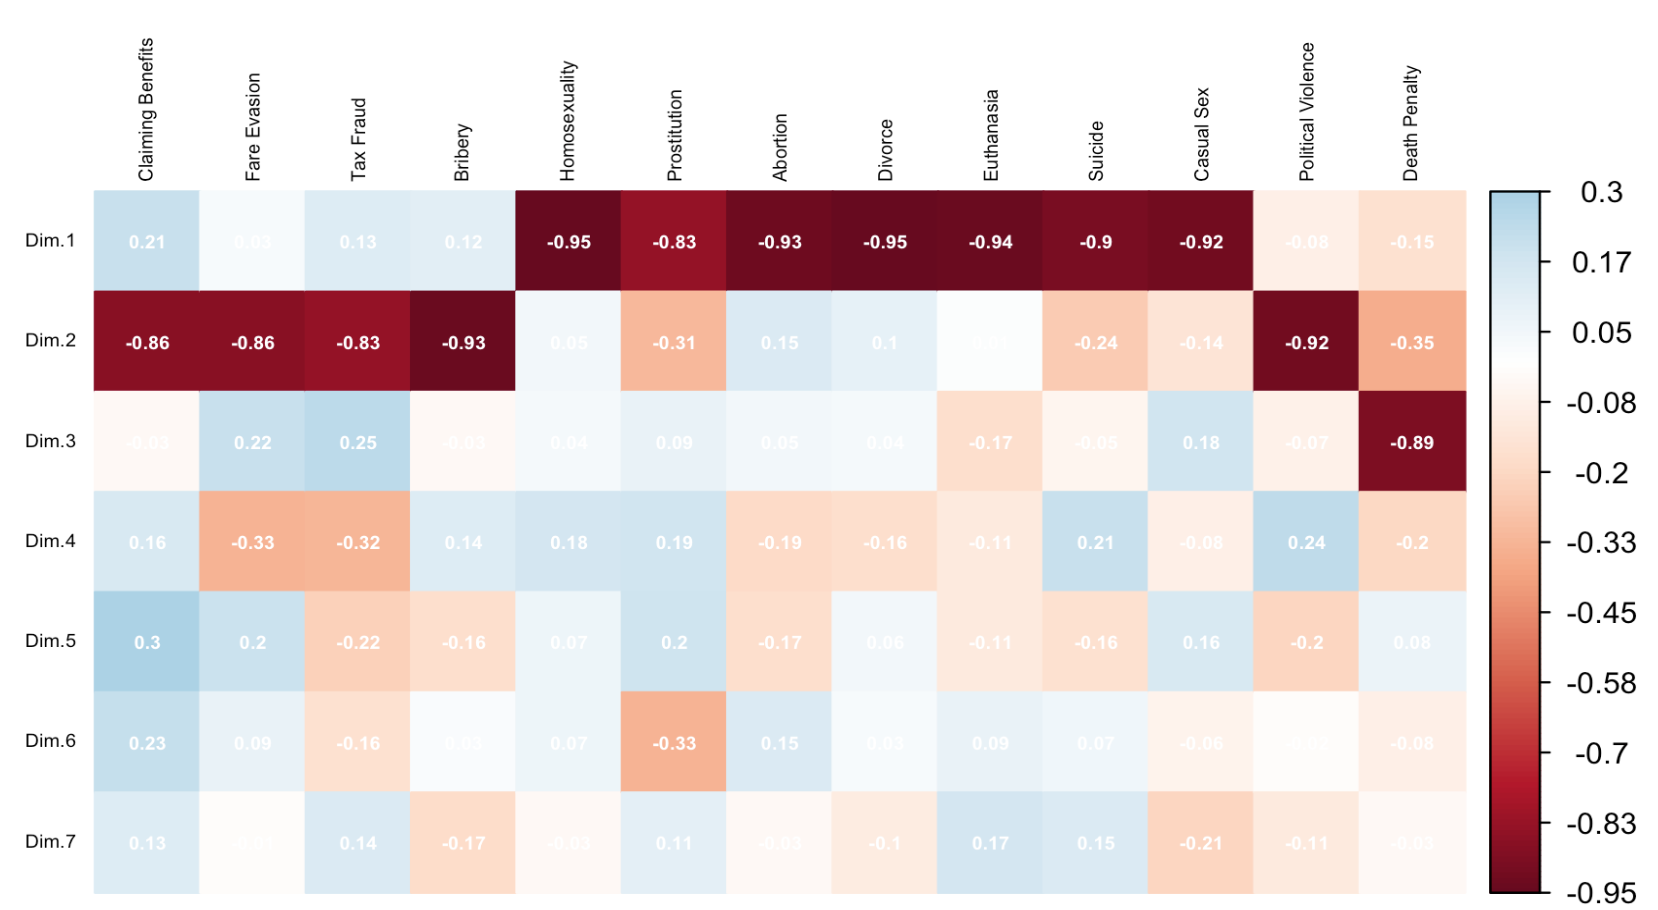
\includegraphics[width=150mm]{cor_Components.png}
    \caption{Correlation of Variable to Components}
    \label{fig:final}
\end{figure}

\begin{table}[ht]
\centering
\caption{Assigned Clusters for each country }
\begin{tabular}{rr}
  \hline
 Country & Cluster Assigned \\ 
  \hline
BG &   1 \\ 
  CN &   1 \\ 
  CZ &   1 \\ 
  EE &   1 \\ 
  FR &   1 \\ 
  GB &   1 \\ 
  HK &   1 \\ 
  HU &   1 \\ 
  JP &   1 \\ 
  PL &   1 \\ 
  TH &   1 \\ 
  TW &   1 \\ 
  US &   1 \\ 
  AR &   2 \\ 
  BO &   2 \\ 
  BR &   2 \\ 
  BY &   2 \\ 
  CL &   2 \\ 
  CO &   2 \\ 
  EC &   2 \\ 
  ES &   2 \\ 
  GT &   2 \\ 
  KR &   2 \\ 
  KZ &   2 \\ 
  LT &   2 \\ 
  MO &   2 \\ 
  MX &   2 \\ 
  MY &   2 \\ 
  PH &   2 \\ 
  RS &   2 \\ 
  RU &   2 \\ 
  SK &   2 \\ 
  UA &   2 \\ 
  VN &   2 \\ 
  AL &   3 \\ 
  AM &   3 \\ 
   \hline
\end{tabular}
\begin{tabular}{rr}
  \hline
 Country & Cluster Assigned \\ 
  \hline
     AZ &   3 \\ 
   BA &   3 \\ 
  BD &   3 \\ 
  CY &   3 \\ 
  ET &   3 \\ 
 GE &   3 \\ 
  HR &   3 \\ 
  ID &   3 \\ 
  KG &   3 \\ 
  ME &   3 \\ 
  MK &   3 \\ 
  MM &   3 \\ 
  NG &   3 \\ 
  NI &   3 \\ 
  PE &   3 \\ 
  PK &   3 \\ 
  PR &   3 \\ 
  PT &   3 \\ 
  RO &   3 \\ 
  TN &   3 \\ 
  ZW &   3 \\ 
  AD &   4 \\ 
  AT &   4 \\ 
  AU &   4 \\ 
  CH &   4 \\ 
  DE &   4 \\ 
  DK &   4 \\ 
  FI &   4 \\ 
  GR &   4 \\ 
  IS &   4 \\ 
  IT &   4 \\ 
  NL &   4 \\ 
  NO &   4 \\ 
  NZ &   4 \\ 
  SE &   4 \\ 
  SI &   4 \\ 
   \hline
\end{tabular}
\label{tab:clusters_Assigned}
\end{table}

\end{document}

